
\section{Exploraci\'on Bivariada}

En este trabajo estamos interesados en el impacto de la cantidad de habitantes en el \'indice de desarrollo humano. Veamos las relaciones bivariadas que tiene esta variable con todas las dem\'as:


% Table created by stargazer v.5.2.2 by Marek Hlavac, Harvard University. E-mail: hlavac at fas.harvard.edu
% Date and time: jue., jul. 05, 2018 - 6:59:25 p.m.
\begin{table}[!htbp] \centering 
  \caption{Correlacion del IDH con la poblacion} 
  \label{corrDem} 
\begin{tabular}{@{\extracolsep{5pt}} cc} 
\\[-1.8ex]\hline 
\hline \\[-1.8ex] 
cabeLog & restoLog \\ 
\hline \\[-1.8ex] 
$0.487$ & $0.177$ \\ 
\hline \\[-1.8ex] 
\end{tabular} 
\end{table} 
Veamos la correlaci\'on entre las variables independientes:

% Table created by stargazer v.5.2.2 by Marek Hlavac, Harvard University. E-mail: hlavac at fas.harvard.edu
% Date and time: jue., jul. 05, 2018 - 6:59:25 p.m.
\begin{table}[!htbp] \centering 
  \caption{Correlacion entre variables independientes} 
  \label{corrTableX} 
\begin{tabular}{@{\extracolsep{5pt}} ccc} 
\\[-1.8ex]\hline 
\hline \\[-1.8ex] 
 & cabeLog & restoLog \\ 
\hline \\[-1.8ex] 
cabeLog & 1 &  \\ 
restoLog & 0.84 & 1 \\ 
\hline \\[-1.8ex] 
\end{tabular} 
\end{table} 
Lo visto en la Tabla \ref{corrTableX} se refuerza claramente en las figuras \ref{corrPlot} y \ref{corrPlotX}.

\begin{figure}[h]
\centering
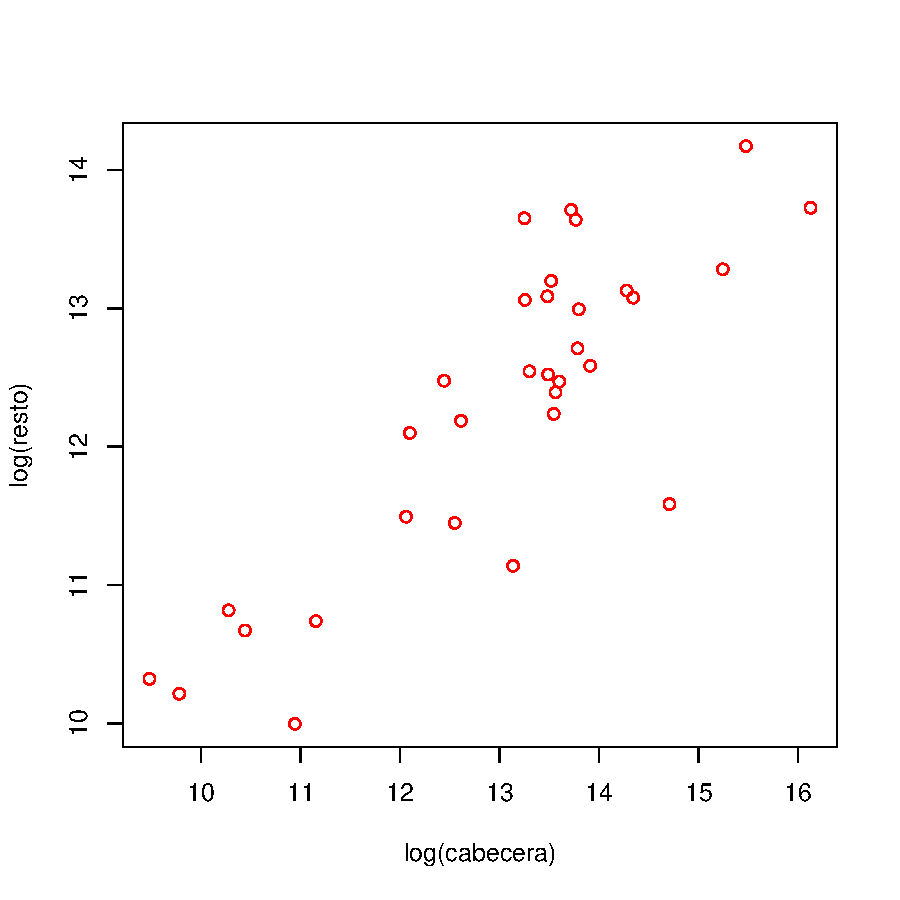
\includegraphics{correlacion-corrPlotX}
\caption{correlacion entre predictores}
\label{corrPlot}
\end{figure}
\endinput
